\section{Progettazione Architetturale}
\textit{Dal 2021-01-18 al 2021-03-01}


\begin{figure}[H]
	\centering
	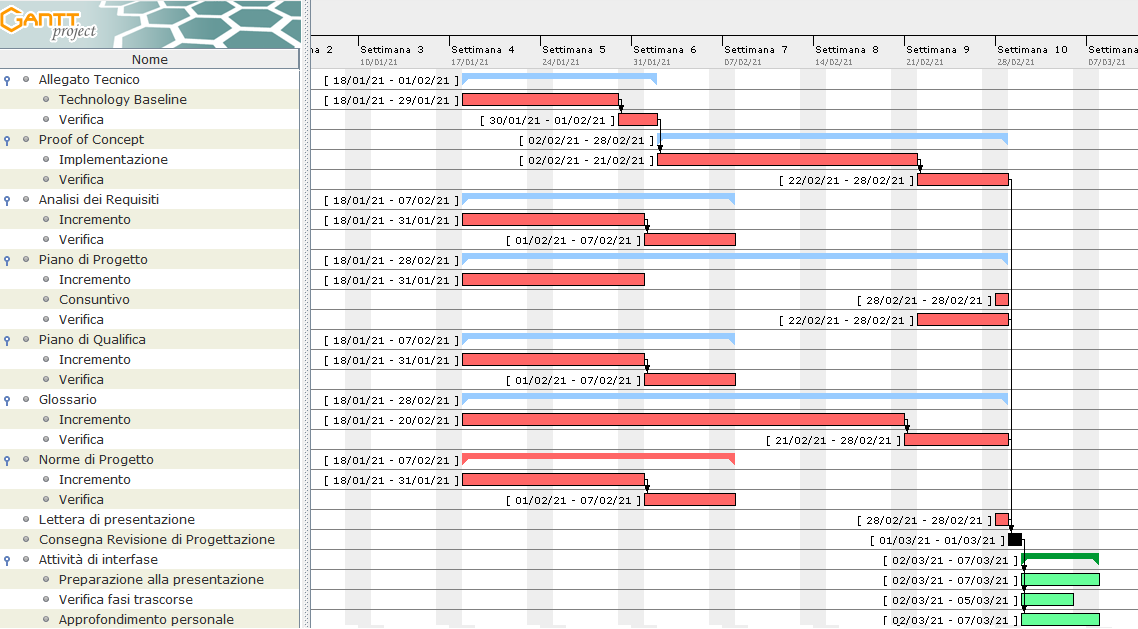
\includegraphics[scale=0.50]{res/images/03_gantt_progettazione.png}
	\caption{Diagramma di gantt\textsubscript{G} relativo alla fase\textsubscript{G} di Progettazione Architetturale}
\end{figure}


\subsection{Periodo 1}

\subsubsection{Pianificazione preventiva}

\paragraph{Attività}

\planningTable{
	Incremento Analisi dei Requisiti & L'avanzamento nello sviluppo del prodotto chiarirà alcuni aspetti che nella fase\textsubscript{G} di Analisi risultavano oscuri, e potrebbe evidenziare delle criticità non inizialmente considerate. Se necessario, viene raffinata l'\textsc{Analisi dei Requisiti} & 8 & Analista
\tabularnewline 
Incremento Piano di Progetto & Il \textsc{Piano di Progetto} viene migliorato fornendo maggior dettaglio, oltre che integrato con il consuntivo del periodo trascorso & 7 & Responsabile
\tabularnewline 
Incremento Glossario & Viene integrato con nuovi termini & 1 & Responsabile
\tabularnewline 
Incremento Piano di Qualifica & Il cruscotto viene aggiornato con i dati rilevati sul periodo trascorso & 16 & Verificatore
\tabularnewline 
\caption{Pianificazione preventiva - Progettazione Architetturale - Periodo 1}
}

\paragraph{Preventivo}


\subsubsection{Pianificazione di periodo}

% gantt @nicolò

\paragraph{Attività}

\planningTable{
	Sistemazione e incremento Analisi dei Requisiti & Nell'Analisi dei Requisiti viene fornito maggior dettaglio a dettagli non inizialmente approfonditi e vengono sistemate alcune criticità riscontrate.  & 8 & Analista
\tabularnewline 
Sistemazione e incremento \textsc{Piano di Progetto} & Il \textsc{Piano di Progetto} viene ristrutturato per rendere più fluente la consultazione e più guidata la pianificazione del progetto. Considerando il tempo risultato necessario a produrre la versione iniziale del documento, il monte orario sarà calibrato al rialzo. & 15 & Responsabile
\tabularnewline 
Incremento \textsc{Piano di Qualifica} & Il \textsc{Piano di Qualifica} viene arricchito e riorganizzato nella suddivisione delle metriche per facilitarne la consultazione. & 20 & Verificatore
\tabularnewline 
Cruscotto interattivo web & Viene predisposto un cruscotto interattivo che faciliti la visualizzazione immediata dell'andamento del progetto, con le nuove metriche presenti nel \textsc{Piano di Qualifica}. Essendo uno strumento nuovo, il monte ore viene stimato al rialzo.  & 10 & Verificatore
\tabularnewline 
\caption{Pianificazione di periodo\textsubscript{G} - Progettazione Architetturale - Periodo 1}
}

\paragraph{Preventivo orario ed economico}



\subsubsection{Riscontro di fine periodo}


\paragraph{Consuntivo orario ed economico}


\paragraph{Preventivo a finire}




\subsection{Periodo 2}

\subsubsection{Pianificazione preventiva}

\paragraph{Attività}

\planningTable{
	Allegato Tecnico & Viene redatto l'\textsc{Allegato Tecnico}, nel quale viene presentata la Technology Baseline, ovvero l'architettura ad alto livello del software. & 62 & Progettista
\tabularnewline 
Setup ambienti di programmazione & Vengono organizzati e messi a punto i software e gli ambienti di sviluppo per i vari linguaggi impiegati. & 6 & Amministratore
\tabularnewline 
PoC - Incremento 1 & Una prima implementazione della soluzione permette di valutarne la bontà: viene realizzato un prototipo del software. Questo incremento riguarda la realizzazione backend del server. & 30 & Programmatore
\tabularnewline 
PoC - Incremento 2 & Realizzazione backend del'unità. & 5 & Programmatore
\tabularnewline 
PoC - Incremento 3 & Realizzazione frontend. & 15 & Programmatore
\tabularnewline 
PoC - Incremento 4 & Collegamento tra frontend e backend. & 10 & Programmatore
\tabularnewline 
Lettera di Presentazione & Avviene la stesura della lettera con cui il gruppo si candida alla Revisione di Progettazione. & 1 & Responsabile
\tabularnewline 
\caption{Pianificazione preventiva - Progettazione Architetturale - Periodo 2}
}

\paragraph{Preventivo}

\subsubsection{Pianificazione di periodo}

% gantt @nicolò

\paragraph{Attività}

\planningTable{
	PoC - Incremento 1.A & Prima implementazione di studio per la comunicazione via socket tra le componenti in Node.js e il server in Java & 25 & Programmatore
\tabularnewline 
PoC - Incremento 1.B & Simulazione della mappa che visualizza le unità sulla base della posizione inviata dalle stesse & 15 & Programmatore
\tabularnewline 
PoC - Incremento 1.C & Definizione semplificata di un algoritmo per la ricerca del miglior percorso per raggiungere la destinazione & 5 & Programmatore
\tabularnewline 
PoC - Incremento 1.D & Ideazione e implementazione di sistema base per la rilevazione e gestione delle collisioni tra le unità & 25 & Programmatore
\tabularnewline 
PoC - Incremento 2 & Realizzazione del backend dell'unità in Node.js e collegamento con il server & 5 & Programmatore
\tabularnewline 
PoC - Incremento 3.A & Presentazione della mappa del magazzino tramite interfaccia realizzata in Angular.js & 20 & Programmatore
\tabularnewline 
PoC - Incremento 3.B & Aggiunta pannello di guida dell'unità nell'interfaccia grafica, e finestra di visualizzazione delle task\textsubscript{G} delle unità & 5 & Programmatore
\tabularnewline 
PoC - Incremento 4 & Collegamento tra server, frontend e unità & 20 & Programmatore
\tabularnewline 
Lettera di Presentazione & Avviene la stesura della lettera con cui il gruppo si candida alla Revisione di Progettazione & 1 & Programmatore
\tabularnewline 
\caption{Pianificazione di periodo\textsubscript{G} - Progettazione Architetturale - Periodo 2}
}


\paragraph{Preventivo orario ed economico}



\subsubsection{Riscontro di fine periodo}


\paragraph{Consuntivo orario ed economico}


\paragraph{Preventivo a finire}





\subsection{Periodo 3}

\subsubsection{Pianificazione preventiva}

\paragraph{Attività}

\planningTable{
	Preparazione alla presentazione & Viene preparato il materiale necessario alla presentazione. & 5 & Amministratore
\tabularnewline 
Verifica dei macro periodi precedenti & Il gruppo si vede coinvolto in un confronto dal quale vorranno emergere le criticità riscontrate nel macro periodo\textsubscript{G} trascorso, al fine di migliorare lo svolgimento dei periodi successivi. & 1 & Responsabile
\tabularnewline 
Approfondimento personale & Ogni membro del gruppo spende alcune ore per formare e consolidare una conoscenza di base degli strumenti e tecniche da impiegare nei periodi successivi. & 5 & Programmatore
\tabularnewline 
\caption{Pianificazione preventiva - Progettazione Architetturale - Periodo 3}
}

\paragraph{Preventivo}


\subsubsection{Pianificazione di periodo}


% gantt @nicolò

\paragraph{Attività}

\planningTable{
	Preparazione alla presentazione & Viene preparato il materiale necessario alla presentazione & 5 & Amministratore
\tabularnewline 
Verifica dei macro periodi\textsubscript{G} precedenti & Il gruppo si vede coinvolto in un confronto dal quale vorranno emergere le criticità riscontrate nel macro periodo\textsubscript{G} trascorso, al fine di migliorare lo svolgimento dei periodi successivi. & 1 & Responsabile
\tabularnewline 
Approfondimento personale & Lo studio personale sarà rivolto alle tecnologie esplorate durante l'implementazione del Proof of Concept, al fine di raffinarne la comprensione e proporre un'implementazione migliorata nella codifica del software & 10 & Programmatore
\tabularnewline 
\caption{Pianificazione di periodo\textsubscript{G} - Progettazione Architetturale - Periodo 3}
}



\paragraph{Preventivo orario ed economico}



\subsubsection{Riscontro di fine periodo}


\paragraph{Consuntivo orario ed economico}


\paragraph{Preventivo a finire}
